\documentclass[letterpaper,preprint,aps,pra,superscriptaddress]{revtex4-1}
\usepackage[T1]{fontenc}
\usepackage[latin9]{inputenc}
\usepackage{units}
\usepackage{amsmath}
\usepackage{amssymb}
\usepackage{graphicx}
\usepackage{wasysym}
\usepackage{braket}

\def\kr{k_{\rm R}}                            				% kr
\def\Er{E_{\rm R}}                            				% kr

\def\ex{\mathbf{e}_x}  
\def\es{\mathbf{e}_s}  
\def\ey{\mathbf{e}_y}  
\def\ez{\mathbf{e}_z}  

\usepackage{babel}
\begin{document}

\title{Diffraction based DMD wavemeter}

\author{I. B. Spielman}
\affiliation{Joint Quantum Institute, National Institute of Standards and Technology,
and University of Maryland, Gaithersburg, Maryland, 20899, USA}

\date{\today}
\begin{abstract}
Here I have some notes describing the physics of a wavemeter based on a DMD.
\end{abstract}
\maketitle

There are two basic types of wavemeters:  using the photon nature of light and using the wave-nature of light.  Generally the latter rely on $E=h\nu$, giving the energy $E$ of a photon of frequency $\mu$ in terms of Planks constant.  The principle of operation is the measure the per-photon energy, for example a bolometer that measures the change in temperature.  I contrast most laboratory wavemeters use some form of interference or wave counting to infer the wavelength or wavenumber. 

\section{Basic operation}

\begin{figure}
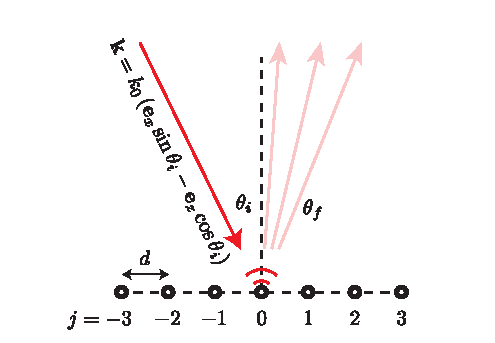
\includegraphics{Schematic}
\caption{Schematic of Bragg scattering from a grating.  An incoming laser with wavevector ${\bf k}_i$ is (possibly) scattered into outgoing beams with wavevector ${\bf k}_f$.}
\label{fig:Grating_Schematic}
\end{figure}

At its core, this device is a grating spectrometer that leverages the angular dependance of Bragg scattering from a diffraction grating to extract the optical wavelength.  Figure~\ref{fig:Grating_Schematic} depicts the basic process of scattering fields off of an array of scatters spaced by a distance $d$ which are infinite along $\ey$.  

\subsection{Bragg Scattering}

I will begin by deriving the relationship between the incident and scattered waves.  We consider an optical field with wavelength $\lambda$ and wavenumber $k_0 = 2\pi/\lambda$ incident at an angle $\theta_i$ on an 1D diffraction grating described by
\begin{align}
E_{\rm init}({\bf x}) &= E_0 \exp\left[i k_0 (\sin\theta_i \ex - E_i \cos\theta_i\ez)\cdot{\bf x} \right]
\end{align}
If we focus on just one element of the grating labeled by $j$, it will produce a scattered field 
\begin{align}
E_i(x,y,z=0) &= E_0 f(x-dj;\theta_i) \exp\left[i k_0 d j \sin\theta_i \right]
\end{align}
at $z=0$.  The first term in this expression $f(x;\theta_i)$ is the scattered field at $z=0$ for an incident field at angle $\theta_i$, in the expression it is evaluated at $x-dj$ the center position of the $j$'th element of the array.  The second term accounts for the position-dependent phase of the incident optical field in the plane of the grating.  Summing these up for all the scatterers gives
\begin{align}
E(x,y,z=0) &= E_0 \sum_j f(x-dj;\theta_i) \exp\left[i k_0 d j \sin\theta_i \right].
\end{align}
At this point we are essentially done, and the last step is to take he Fourier transform of this expression
\begin{align}
\tilde E({\bf k}_{\rm 2D},z=0) &= E_0 \sum_j \int d^2 {\bf x}_{\rm 2D} f(x-dj;\theta_i) \exp\left[i (k_0 d j \sin\theta_i - {\bf k}_{\rm 2D}\cdot{\bf x}_{\rm 2D}) \right] \\
&= E_0 \sum_j \int d^2 {\bf x}_{\rm 2D} f(x;\theta_i) \exp\left\{i [(k_0 \sin\theta_i - k_x) d j - {\bf k}_{\rm 2D}\cdot{\bf x}_{\rm 2D}] \right\}\\
&= E_0 \tilde f({\bf k}_{\rm 2D};\theta_i) \sum_j \exp\left[i (k_0 \sin\theta_i - k_x) d j \right].
\end{align}
There is just one more step, but I wanted to comment at this point that the overall form-factor $\tilde f({\bf k}_{\rm 2D};\theta_i)$ is now controlling the overall shape of the scattered field (which is why it is called a form-factor).  Last, we sum over all of elements of the grating, which in the infinite limit produces a chain of delta functions describing outgoing orders labeled by $\ell$
\begin{align}
\tilde E({\bf k}_{\rm 2D},z=0) &\propto \tilde f({\bf k}_{\rm 2D};\theta_i) \sum_\ell \delta[(k_0 \sin\theta_i - k_x) d - 2\pi\ell].
\end{align}
Thus we find scattered beams when $(k_0 \sin\theta_i - k_x) d = 2\pi\ell$, since we know that $k_y=0$ (this will be from the form factor, which will take the form $\tilde f({\bf k}_{\rm 2D};\theta_i) = \tilde f(k_x;\theta_i) \delta(k_y)$ because it was independent of $y$ in coordinate space.  To finish the story, we know that the total wavenumber is $k_x^2 + k_z^2 = k_0^2$ so we can dived our scattering condition by $k_0$ to arrive at the Bragg condition
\begin{align}
\sin\theta_i - \frac{k_x}{k_0} =\sin\theta_i - \sin\theta_f &= \ell \frac{\delta k}{k_0} = \ell\frac{\lambda}{d}, & {\rm with} && \delta k &= \frac{2\pi}{d}.
\end{align}
And that is it.

\subsection{Sensitivity}

Any possible utility of this device rests on the observable change in angle resulting from a change in wavelength.  We will consider a detection approach where we place a lens of focal length $f$ a distance $f$ away from the grating and measure the spatial displacement of a specific order in response to the change in wavelength. 

Linearizing around very small fractional wavelength changes we have
\begin{align}
\frac{d x}{d \lambda} &= -\frac{\ell f}{d\cos\theta_f} = -\frac{\ell f}{d}\left[1-\left(\sin\theta_i+\frac{\ell \lambda}{d}\right)^2\right]^{-1/2}
\end{align}


\begin{acknowledgments}
This work was partially supported by ...
\end{acknowledgments}

\bibliographystyle{apsrev4-1}
% \bibliography{StripePhase}

\end{document}
